\documentclass{article}
\usepackage{graphicx}

\title{Lisc Python Package}
\author{Katie Brown}
\date{August 4,2020}

\begin{document}

\maketitle

\section{Introduction}

Lisc collects and analyzes data form the NCIB database. This data can be counts and co-occurrences of search terms in the literature, text data and meta-data from articles that contain the search terms and can be used to collect citation data from DOIs. This data can be managed through data objects, saved, loaded and ploted.

\section{Data}
Using this package you can collect the counts data for the word co-occurrence data between terms as seen in ~\ref{fig:1}.

% 
\begin{figure} 
  \centering 
  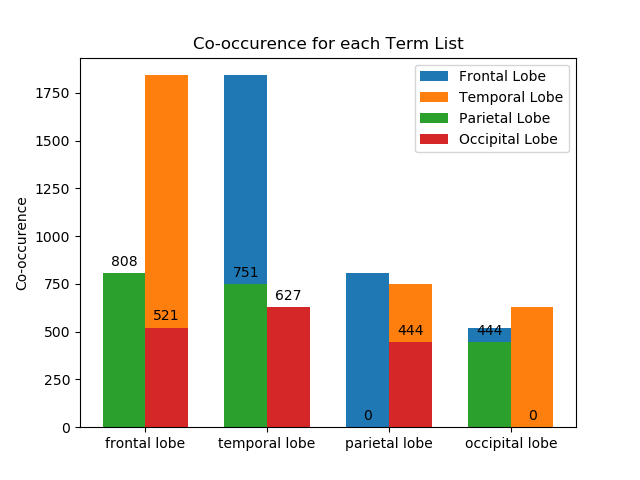
\includegraphics[width=0.9/textwidth]{counts.png}
  \caption{Matplotlib bar graph of the number of counts for word co-occurrence in the search term list.} 
  \label{fig:1}
\end{figure}
%

We can also look at how many articals contain each of the specified search terms ~\ref{fig:2}
%
\begin{figure}
  \centering
  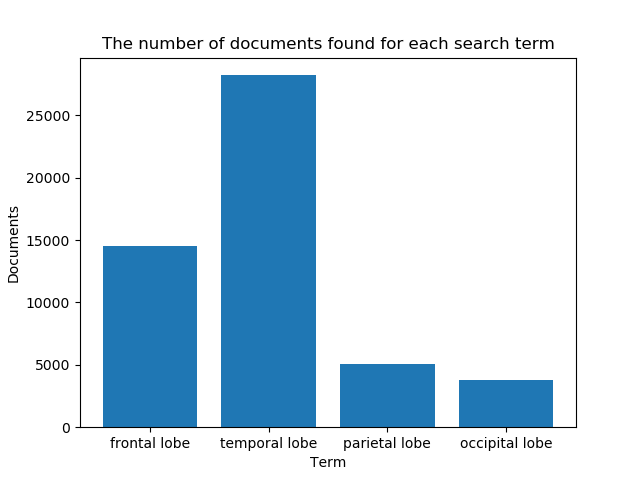
\includegraphics[width=0.9/textwidth]{document.png}
  \caption{Matplotlib bar graph of the number of documents found for each search term.}
  \label{fig:2}
\end{figure}
%
Another example of this packages function is it's ability to change NCIB databases, the above figures used the Pubmed database and ~\ref{fig:3} uses the Nucleotide database. The example searched for five orgainisms and returned the number of articles that contained the search terms.
%
\begin{figure}
  \centering
  
\includegraphics[width=0.9/textwidth]{organism.png}
  \caption{Matplotlib graph of th e number of articles that contain "Salmonella enterica" "Escherichia coli" "Sus scrofa" "Homo sapiens" and "Mus musculus".}
  \label{fig:3}
\end{figure}
%
\section{Conclusions}

Lisc is a great tool to collect data on articles using several databases. It can plot the data in various ways.

\section{Reference}

Donoghue, T. (2018) LISC: A Python Package for Scientific Literature Collection and Analysis. Journal of Open Source Software, 4(41), 1674. DOI: 10.21105/joss.01674

\end{document}
